\documentclass{article}

\PassOptionsToPackage{numbers,compress}{natbib}
\usepackage[UTF8,fontset=none,heading=false]{ctex}
\setCJKmainfont[AutoFakeBold=2.5,ItalicFont={Songti SC},SmallCapsFont={Songti SC}]{Songti SC}
\setCJKsansfont[AutoFakeBold=2.5]{Hiragino Sans GB}
\setCJKmonofont[Scale=0.92]{Songti SC}
\setmainfont{texgyretermes-regular.otf}[
  BoldFont=texgyretermes-bold.otf,
  ItalicFont=texgyretermes-italic.otf,
  BoldItalicFont=texgyretermes-bolditalic.otf
]
\setsansfont{texgyreheros-regular.otf}[
  BoldFont=texgyreheros-bold.otf,
  ItalicFont=texgyreheros-italic.otf,
  BoldItalicFont=texgyreheros-bolditalic.otf
]
\setmonofont{texgyrecursor-regular.otf}[
  BoldFont=texgyrecursor-bold.otf,
  ItalicFont=texgyrecursor-italic.otf,
  BoldItalicFont=texgyrecursor-bolditalic.otf,
  Scale=MatchLowercase
]
\XeTeXlinebreaklocale "zh"
\XeTeXlinebreakskip = 0pt plus 1pt

\usepackage{iclr2026_conference}
\input{math_commands.tex}

\usepackage{hyperref}
\usepackage{url}
\usepackage{graphicx}
\usepackage{colortbl}
\usepackage{wrapfig}
\usepackage{multirow}
\usepackage{makecell}
\usepackage{caption}
\usepackage{cleveref}
\usepackage{tcolorbox}
\usepackage[subrefformat=parens]{subcaption}
\tcbuselibrary{breakable}
\usepackage{stfloats}
\usepackage{booktabs}
\usepackage{xspace}

\hypersetup{colorlinks,linkcolor={red},citecolor={blue},urlcolor=orange}
\definecolor{COLOR_MEAN}{HTML}{f0f0f0}
\definecolor{LIGHT_BLUE}{HTML}{e6f1fe}
\definecolor{LIGHT_RED}{HTML}{fceeee}
\definecolor{LIGHT_YELLOW}{HTML}{f1f58a}
\definecolor{LIGHT_GREEN}{HTML}{eaffea}
\definecolor{LIGHT_BROWN}{HTML}{f5e6d3}
\newcommand{\ie}{\textit{i.e.},\xspace}
\newcommand{\eg}{\textit{e.g.},\xspace}
\renewcommand{\figurename}{图}
\renewcommand{\tablename}{表}
\renewcommand{\refname}{参考文献}
\captionsetup[figure]{name=图}
\captionsetup[table]{name=表}
\crefname{figure}{图}{图}
\Crefname{figure}{图}{图}
\crefname{table}{表}{表}
\Crefname{table}{表}{表}
\crefname{section}{第}{第}
\Crefname{section}{第}{第}
\crefname{equation}{式}{式}
\Crefname{equation}{式}{式}
\setlength{\emergencystretch}{2em}

\title{Task-CoEvolve：通过自适应验证任务选择实现高效 Harness 优化}

\author{
Atsuyuki Miyai\hspace{0.8em}
Kiyoharu Aizawa\thanks{共同指导本研究。}\hspace{0.8em}
Toshihiko Yamasaki\footnotemark[1] \\[1ex]
东京大学 \\
\texttt{miyai@cvm.t.u-tokyo.ac.jp}
}

\iclrfinalcopy
\begin{document}

\maketitle

\begin{figure*}[h]
\vspace{-25pt}
\centering
    
\includegraphics[width=0.95\linewidth]{figs/teaser.pdf}\\
    \vspace{-5pt}
   \caption{\textbf{现有 harness 优化方法与本文 Task-CoEvolve 的对比。}}
    \label{fig:fig_teaser}
\end{figure*}

\begin{abstract}
本文提出一种通过自适应选择验证任务来高效优化大语言模型（LLM）harness 的新方法。Harness 优化会依据验证性能迭代重写 harness 代码，从而在不更新底层模型权重的情况下显著提升性能。然而，现有方法在每次迭代中都会完整评估一组固定的验证任务；即便随着 harness 演化，某些任务已不再具有足够区分力，仍会产生大量评估开销。我们提出 \textbf{Task-CoEvolve}，通过解决两个挑战，让验证任务与 harness \emph{共同演化}：一是选择信息量高的任务，二是利用部分评估估计全任务集性能。Task-CoEvolve 基于这样一个观察：相比始终被成功解决或始终失败的任务，候选 harness 结果存在分歧的任务更有助于区分这些候选方案。该方法依据历史结果进行方差加权采样，使评估聚焦于能力前沿附近的任务，并随着 harness 演化自适应地调整采样分布。随后，它在估计全任务集分数时考虑被采样任务各自的采样概率，因此即使不同迭代评估了不同子集，也能进行一致的比较。在线文本分类和 Terminal-Bench 2.1 上的实验表明，Task-CoEvolve 始终优于基于子集的基线，并在优化期间将评估次数减少 80\% 的同时达到全任务集搜索的最终性能。代码将发布于 \url{https://github.com/Agent4Science-UTokyo/Task-CoEvolve}。
\end{abstract}

\section{引言}

将 LLM 智能体部署到真实世界任务时，harness（执行脚手架）的设计至关重要；它是决定存储什么、检索什么以及向模型呈现什么内容的代码。已有研究表明，仅改变固定 LLM 外围的 harness，就能在同一基准上造成最高 $6\times$ 的性能差异~\citep{Tian2026SWEBenchMC}，这说明 harness 的重要性可能不亚于底层模型本身。传统上，harness 由人工设计~\citep{zhang2025ace, ye2026meta, merrill2026terminal, terminuskira2026}，但其设计空间庞大，使这一过程成本高昂且高度依赖大量试错。近期，\emph{自动化 harness 优化}开始受到广泛关注：元层智能体迭代重写 harness 代码，在基准上评估所得候选方案，并保留能够提升性能的修改~\citep{lee2026meta, lin2026agentic, zhang2026harnessing, wang2026rethinking, guo2026drevo, weng2026harness}。

然而，现有自动化 harness 优化工作大多采用朴素的评估策略：在每次迭代中，都用整个\emph{固定}验证任务集评估每个候选 harness~\citep{lee2026meta, lin2026agentic, zhang2026harnessing, wang2026rethinking}。这种策略实现简单，也便于直接比较候选方案，但存在两个关键局限。第一，成本高。每次迭代都必须在完整验证集上进行推理；当单项任务执行代价很高时，例如需要占用沙箱环境数十分钟的长时程终端任务~\citep{merrill2026terminal}，评估可能成为整个优化循环的主要成本。第二，它是\emph{静态的}。随着 harness 演化，能够有效区分候选方案的任务也会变化。所有候选方案都已能解决的任务，或者所有候选方案尚且无法解决的任务，仍会消耗评估预算，却几乎不提供优化信号。要克服这些局限，就必须在评估成本与所得优化信号的信息量之间取得平衡，并让验证任务本身随 harness 一同演化。

本文研究如何在每次迭代中仅使用验证任务子集，高效开展 harness 优化。我们提出 \textbf{Task-CoEvolve}，使验证任务集与 harness \emph{共同演化}（\Cref{fig:fig_teaser}）。Task-CoEvolve 解决两个挑战：（i）选择最能区分候选 harness 的任务；（ii）尽管各次迭代使用不同子集，仍使评估结果彼此可比。对于（i），我们观察到，候选方案结果不同的任务信息量更高，而始终成功或始终失败的任务几乎无法帮助候选排序。我们用各任务历史成功率的伯努利方差衡量这一点：成功与失败较为均衡时，该方差较大。随着 harness 演化，采样分布也相应变化，以聚焦于对当前 harness 具有信息量的任务。对于（ii），我们使用任务纳入概率，根据每次采样的子集估计全任务集分数，为不同迭代提供共同的评估标准。两部分结合后，便可将评估集中在信息量高的任务上，同时无需每次迭代都评估完整验证集，也能公平比较并选出最终方案。

按照既有工作~\citep{lee2026meta}，我们在在线文本分类~\citep{fei2024lawbench, gretel2023symptom, schneider2016s}和面向长时程终端智能体的基准 Terminal-Bench 2.1~\citep{merrill2026terminal}上评估 Task-CoEvolve。在文本分类中，即使评估预算极低、仅为 7\%，Task-CoEvolve 也接近全任务集搜索；当评估预算为 20\% 时，它甚至超过全任务集搜索。在 Terminal-Bench 2.1 上，Task-CoEvolve 只使用 20\% 的评估次数便达到全任务集搜索的性能，同时将总体搜索成本降低 67--80\%。
我们的贡献概括如下：
\begin{itemize}
\item \textbf{问题设定。} 我们提出一个新问题：优化用于评估候选 harness 的\emph{任务选择}。此前的效率方法通过减少候选方案数量来降低成本，而本方向与之正交，着眼于减少每个候选方案的评估成本。

\item \textbf{Task-CoEvolve。} 我们提出 Task-CoEvolve，将基于区分力的自适应任务选择与根据部分评估估计全任务集分数相结合（\Cref{fig:fig_teaser}）。前者把评估预算集中到能力前沿附近，后者则为不同子集提供共同的评估标准。

\item \textbf{实证发现。} 在文本分类中，Task-CoEvolve 仅用 7\% 的评估预算便接近全任务集搜索，并在 20\% 预算下超过后者（\Cref{table:tc}）。在 Terminal-Bench 2.1 上，它在取得相近性能的同时将搜索成本降低 67--80\%。
\end{itemize}

\section{相关工作}
\label{sec:related_work}

\textbf{Harness 的自动优化。}
递归自我改进研究传统上着眼于通过更新权重来改进模型本身~\citep{huang-etal-2023-large, pmlr-v235-yuan24d, NEURIPS2025_6b41e04c, NEURIPS2022_639a9a17}。近期，研究关注点开始转向在底层模型保持固定的情况下改进 harness~\citep{lee2026meta, lin2026agentic, nie2026tthe, zhang2026harnessing}。这些方法通过反复提出 harness 修改、评估所得候选方案并采纳有前景的变化，逐步改进 harness。Meta-Harness~\citep{lee2026meta} 是一个代表性例子：它在给定任务集上评估多个 harness 候选方案，利用这些方案的执行轨迹与性能历史迭代改进 harness，最终以最大化目标任务分布上的性能为目标。然而，这些方法~\citep{lee2026meta, lin2026agentic, zhang2026harnessing}共有一个局限：每次迭代都会在完整的验证任务集上重复评估候选 harness。因此，评估可能带来巨大的计算与时间开销，尤其是在单项任务本身执行代价高昂时。

\textbf{高效 Harness 优化。}
近期工作从若干方向探索了如何提升 harness 与程序优化的效率。DemoEvolve~\citep{che2026demoevolve} 引入人类示范，为稀疏奖励场景提供信息量更高的反馈；ShinkaEvolve~\citep{lange2025shinkaevolve} 和 TurboEvolve~\citep{yang2026turboevolve} 则借助更高效的候选生成与选择策略，提高 LLM 驱动进化搜索的样本效率。HarnessCompass~\citep{zhang2026harnesscompass} 进一步通过带约束、反馈引导和组件级优化来改进 harness 演化。这些方法主要提高搜索侧的效率，例如更有效地生成、选择或细化候选 harness。本文处理另一项与其正交的成本来源：评估每个候选方案所用的任务数量。Task-CoEvolve 通过降低单个候选方案的评估成本，与上述方法形成互补。

\textbf{课程学习与自适应任务选择。}
课程学习和自适应任务选择会根据模型当前能力动态选择训练任务，以提高学习效率与性能~\citep{bengio_curriculum, ruvolo2013active, soviany2022curriculum}。概括而言，这些方法优化的是\emph{从什么内容学习}。相比之下，harness 优化的关键问题是\emph{在什么内容上评估}。训练任务为更新模型参数提供监督，而 harness 优化中的评估任务决定更偏好哪些候选 harness，从而引导优化方向。

\textbf{样本高效的模型评估。}
既有研究通过在选定测试样例上估计模型性能来降低评估成本。主动测试会有选择地评估信息量高的测试样例，并以重要性加权方式估计性能~\citep{kossen21a2021active}。tinyBenchmarks~\citep{polo2024tiny} 和 AcTracer~\citep{huang2026actracer} 分别借助紧凑的基准子集和模型感知采样，进一步提高 LLM 评估的样本效率。这些方法主要关注如何高效估计固定模型的性能。相较之下，Task-CoEvolve 选择任务的目的是区分不断演化的 harness 候选方案，并在估计全任务集性能时校正非均匀采样。

\begin{figure*}[t]
\vspace{-25pt}
\centering
    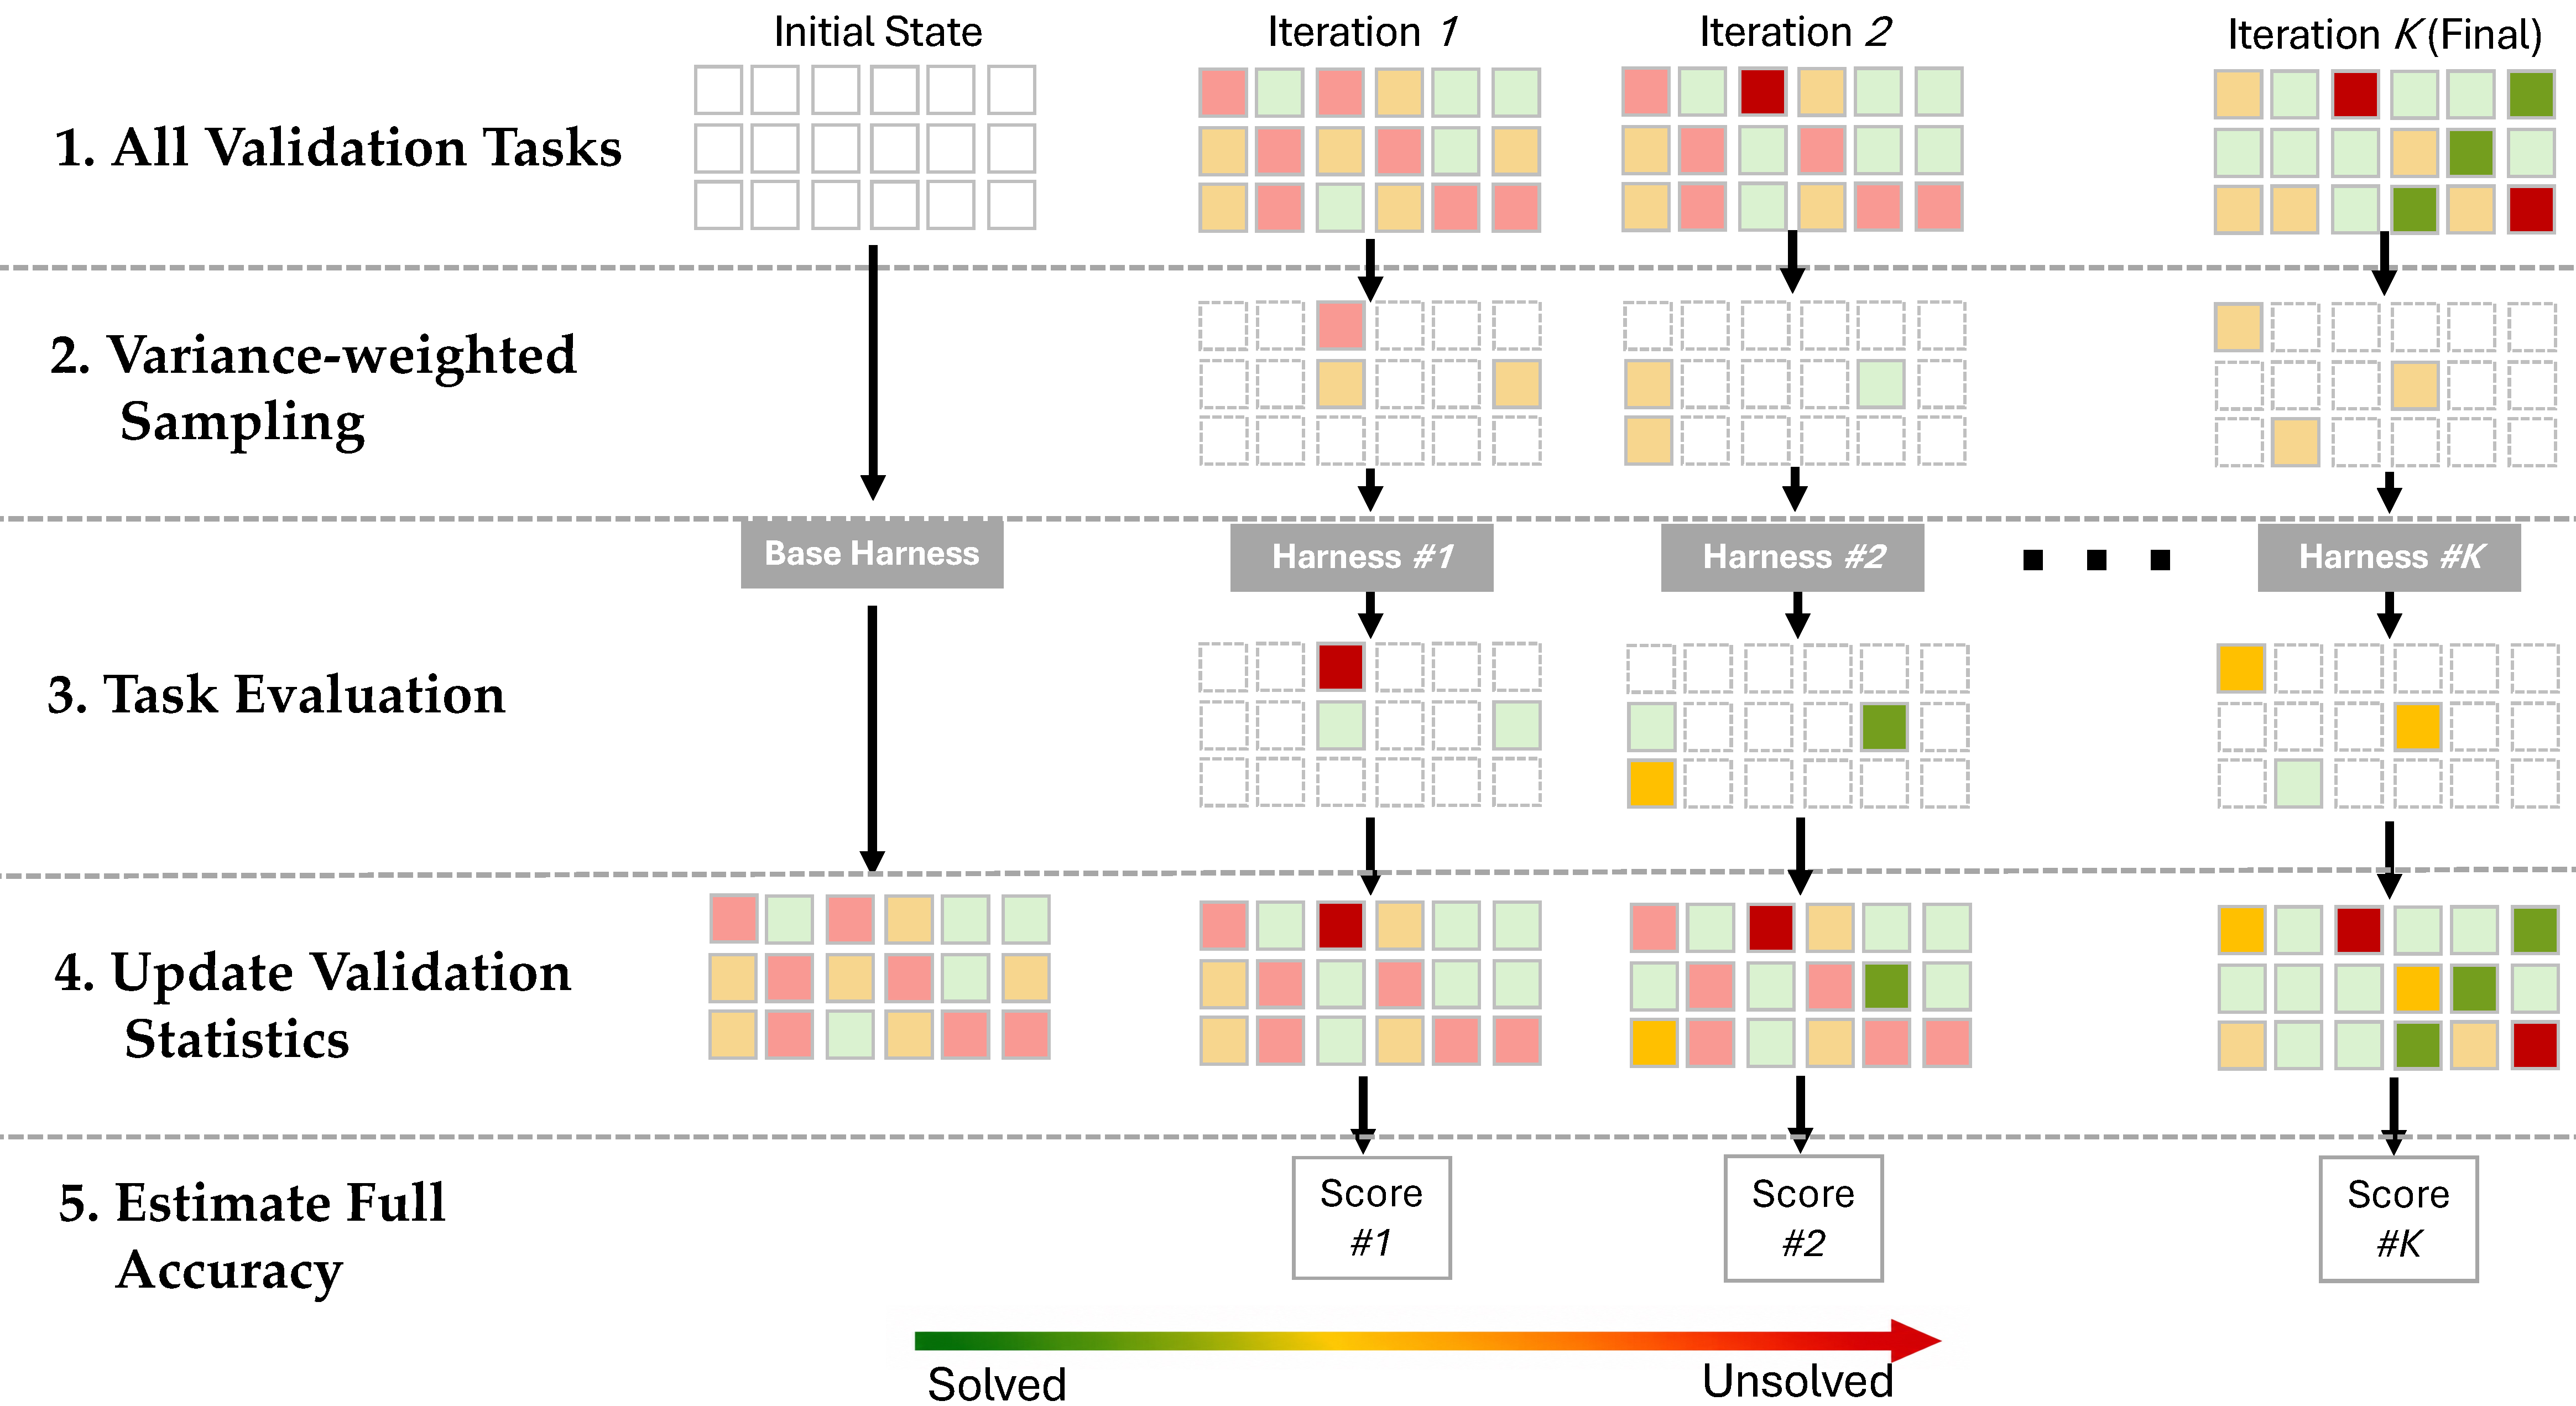
\includegraphics[width=0.95\linewidth]{figs/taskevole_details.pdf}\\
    \vspace{-5pt}
\caption{\textbf{Task-CoEvolve 流程概览。}Task-CoEvolve 首先用方差加权采样从完整验证集中选择任务子集，并在所选任务上评估候选 harness。所得结果用于更新验证任务统计量。最后，Task-CoEvolve 根据采样评估估计全任务集准确率。}
    \label{fig:overview}
\end{figure*}

\section{方法}
\label{sec:method}

\subsection{问题定义}

我们考虑一个固定的 LLM 和一个 \textit{harness} $h$，即围绕模型的控制代码。令 $\mathcal{T}=\{1,\dots,N\}$ 表示验证任务集，令 $x_t(h)\in[0,1]$ 表示 harness $h$ 在任务 $t\in\mathcal{T}$ 上经过 $r$ 次试验后的平均成功率。我们将 harness $h$ 的真实性能定义为其全任务集分数：
\begin{equation}
\begin{aligned}
S(h) = \frac{1}{N} \sum_{t \in \mathcal{T}} x_t(h).
\end{aligned}
\label{eq:full_set_score}
\end{equation}

在 harness 优化中，元层智能体在每次迭代 $k=1,\dots,K$ 根据先前的评估结果提出候选 harness $h_k$，并把新结果反馈给后续迭代。目标是在优化期间生成的全部候选方案中，选出 $S(h)$ 最高的 harness。本文考虑如何在有限的评估预算下实现这一目标；预算以任务执行总次数衡量。

重要的是，我们的任务选择和全任务集估计过程只依赖观测到的任务结果，即成功与失败的历史，而不对任务内容或 harness 代码作任何假设。

\subsection{Meta-Harness 回顾}
\label{subsec:review_meta_harness}

Meta-Harness~\citep{lee2026meta} 是自动化 harness 优化的代表性框架。在每次迭代中，元智能体接收先前的 harness 候选方案及其评估结果作为上下文，并生成新 harness $h_k$ 的代码。随后在\emph{整个}验证任务集 $\mathcal{T}$ 上评估候选方案 $h_k$，并记录其平均分数 $\frac{1}{N}\sum_{t \in \mathcal{T}} x_t(h_k)$。经过 $K$ 次迭代后，选择记录分数最高的候选方案作为最终 harness。该过程共需执行 $K \times N \times r$ 次任务，每次迭代都会产生与 $N$ 成正比的评估成本。

\subsection{所提方法：Task-CoEvolve}
\label{subsec:proposed_approach}

一种自然的降本方式，是只在大小为 $m = \lceil \rho N \rceil$ 的子集 $\mathcal{S}_k \subset \mathcal{T}$ 上评估每个候选方案，从而把任务执行次数由 $K \times N \times r$ 降至 $K \times m \times r$。但这带来两个挑战。重复使用固定子集会诱发过拟合，因为元智能体会不断偏好只在同一批任务上奏效的修改。每次迭代重新采样虽可避免这一问题，但原始子集均值会受到所采任务难度的影响，因而不同迭代的分数不再可比。

\textbf{总体思路。}
Task-CoEvolve 用两个组件解决上述挑战。第一，\emph{方差加权任务选择}依据过去的评估结果，在每次迭代中选择新的验证子集，使评估预算集中于信息量高的任务。第二，\emph{全任务集分数估计}在考虑采样概率的前提下，根据采样任务估计全任务集性能~\citep{Horvitz01121952}。这样便能用同一尺度比较在不同子集上评估的候选方案。\Cref{fig:overview} 展示了总体流程。

\textbf{阶段 0：初始化。}
搜索开始前，我们在完整任务集 $\mathcal{T}$ 上评估两个初始 harness。这些运行并非本文方法的额外成本：harness 优化无论如何都需要它们，因为元智能体会在二者基础上编写第一个候选方案。我们复用其结果作为初始历史，使第一次抽取子集时，每项任务都已有成功率 $\bar{p}_t$。

\textbf{阶段 1：方差加权任务选择。}
我们用一个简单标准衡量每项任务的信息量：其历史结果的伯努利方差。先前 harness 在某项任务上的结果不同时，该方差会变大。在迭代 $k$，令 $\bar{p}_t$ 和 $n_t$ 分别表示此前迭代中观测到的任务 $t$ 结果均值与结果数量。我们如下定义任务 $t$ 的采样权重：
\begin{equation}
\begin{aligned}
w_t = \max\bigl( \bar{p}_t (1 - \bar{p}_t),\; \ell_t \bigr) + \frac{\lambda}{\sqrt{n_t}}.
\end{aligned}
\label{eq:vws_weight}
\end{equation}
第一项表示伯努利方差，它在 $\bar{p}_t=0.5$ 时最大，在任务始终成功或始终失败时为零。对于从未被解决的任务，下界 $\ell_t$ 等于一个很小的正常数 $\ell$；否则为 $0$。之所以保留这一正下界，是因为当前无人解决的任务仍可能随着 harness 改进而变得可解。第二项 $\lambda/\sqrt{n_t}$ 为观测较少的任务赋予更大权重，避免仅根据少量早期结果便将其排除。

\textbf{阶段 2：采样感知的全任务集估计。}
为了在不同迭代间进行公平比较，我们根据采样任务估计全任务集性能。核心思想是考虑采样设计下每项任务的纳入概率 $\pi_t = \Pr[t \in \mathcal{S}_k]$~\citep{Horvitz01121952}；本文通过蒙特卡洛模拟估计该概率。然而，我们发现，适当的全任务集估计形式取决于各基准任务池的结构（详细实验见原文附录 A）。因此，在阶段 0 的评估和任务集类型指引下，我们为每个基准采用以下两种估计量之一。

\textbf{\textit{成功率接近 $0$ 或 $1$ 时采用 H\'ajek 估计。}}
用 $1/\pi_t$ 对每个采样结果加权，可得 H\'ajek 估计量~\citep{hajek1964asymptotic}：
\begin{equation}
\begin{aligned}
\hat{S}(h) = \frac{\sum_{t \in \mathcal{S}_k} x_t(h) / \pi_t}{\sum_{t \in \mathcal{S}_k} 1 / \pi_t}.
\end{aligned}
\label{eq:full_estimate}
\end{equation}
该形式适用于满足以下条件的任务集：（i）任务集可拆成若干任务池，各池分别采样和估计，再对结果取平均；（ii）每个任务池内的平均成功率都接近 $0$ 或 $1$，因为此时罕见被采样任务的结果会接近其所在任务池的均值。

\textbf{\textit{成功率接近中间区域时采用锚定差值估计。}}
否则，一项始终成功且 $\pi_t$ 极小的任务偶尔被采中时，其 $x_t(h)/\pi_t$ 项会主导\Cref{eq:full_estimate}。因此，我们不对结果本身加权，而是对其相对于\emph{锚点} $\bar{p}_t$ 的偏差加权；这里的锚点是任务 $t$ 的历史成功率：
\begin{equation}
\begin{aligned}
\hat{S}(h) = \frac{1}{N}\sum_{t \in \mathcal{T}} \bar{p}_t \;+\; \frac{1}{N}\sum_{t \in \mathcal{S}_k} \frac{x_t(h) - \bar{p}_t}{\pi_t}.
\end{aligned}
\label{eq:difference}
\end{equation}
锚点在采样前固定，因此在期望中会相消。

\textbf{阶段 3：最终选择。}
优化结束后，我们选择估计全任务集分数 $\hat{S}(h)$ 最高的候选方案作为最终 harness；若分数完全相同，则优先选择更早的迭代。关于平局规则的额外实验见原文附录 B。

\section{实验}
\label{sec:experiments}

按照 \citet{lee2026meta}，我们在两类设定中进行评估。首先使用在线文本分类对 Task-CoEvolve 进行严格验证，并通过全面实验精确量化其收益。随后使用 Terminal-Bench 2.1~\citep{merrill2026terminal}，检验这些发现能否推广到真实且计算密集的场景。

\subsection{在线文本分类设定}
\textbf{基准与实现细节。}
我们沿用 \citet{zhang2025ace,ye2026meta,lee2026meta} 的在线文本分类设定：LLM 每次接收一个带标签样例，更新其记忆（harness），随后在留出测试集上接受评估。按照 \citet{lee2026meta}，我们使用温度为 $0$ 的 \texttt{GPT-OSS-120B}~\citep{agarwal2025gpt} 作为分类器 LLM，并自动优化其 harness。我们采用三个领域与难度各异的数据集：\textbf{LawBench}（Law）~\citep{fei2024lawbench}，根据案件描述预测刑事罪名（215 类）；\textbf{Symptom2Disease}（S2D）~\citep{gretel2023symptom}，根据症状描述预测疾病（22 类）；以及 \textbf{USPTO-50k}~\citep{schneider2016s}，根据产物分子预测前体反应物（180 类）。Law、S2D 和 USPTO 的训练/验证/测试划分分别为 200/50/100、200/50/212 和 50/30/100，共得到 $N=130$ 个验证样例和 412 个测试样例。

按照 Meta-Harness，我们使用 Claude Opus 4.6~\citep{anthropic2026claudeopus46} 作为元智能体，运行 20 次演化迭代；每次迭代生成三个候选 harness，共 60 个候选方案。为研究评估预算的影响，我们在验证集采样率 $\rho \in \{7\%, 20\%\}$ 下分别运行每种方法。每个设定运行三次，并报告最终所选 harness 在留出测试集上的准确率，再对三个数据集取平均。

\textbf{基线与比较方法。}
我们使用 Meta-Harness~\citep{lee2026meta} 作为基础搜索框架。Meta-Harness 是自动化 harness 优化的代表性框架（\Cref{subsec:review_meta_harness}）；其结构简单、扩展性强，适合比较不同评估设计。按照 Meta-Harness 官方实现，所有演化流程都从两个初始 harness 出发：零样本（不使用记忆、直接提示）和少样本（全部）（把全部训练样例放入上下文）。

我们考虑三种演化方法：\textbf{（1）Meta-Harness（全任务集搜索）}是原始流程~\citep{lee2026meta}，每次迭代都评估完整验证集（$\rho=100\%$）；\textbf{（2）Naive} 在搜索开始时采样一个固定子集，并在所有迭代中重复使用该子集，最终选择原始子集分数最高的候选方案；\textbf{（3）Random-Resample} 在每次迭代中从 $\mathcal{T}$ 随机重采样子集 $\mathcal{S}_k$，但仍使用子集分数作最终选择。该基线有助于区分两类效应：一类只是改变评估子集以减少过拟合，另一类来自本文方法中的判别性选择与采样感知估计。这里的分数按数据集分别估计，\Cref{subsec:proposed_approach} 的规则为该设定分配 H\'ajek 估计量（\Cref{eq:full_estimate}；阶段 0 的依据见原文附录表 C）。

\subsection{在线文本分类结果}
\label{subsec:result_text-classification}
\Cref{table:tc} 给出了结果。主要发现如下。
\begin{table}[t]
\centering
\caption{\textbf{在线文本分类。}各流程在评估预算 $\rho$ 下所选 harness 的留出测试准确率。``每轮验证''：每次迭代的验证样本数（USPTO/S2D/Law）；``评估数''：搜索期间的样本评估总数。\dag：\citet{lee2026meta} 报告的数值。Task-CoEvolve 在 $\rho{=}7\%$ 时几乎追平全任务集搜索，在 $\rho{=}20\%$ 时超过后者。}
\label{table:tc}
\small
\setlength{\tabcolsep}{4.5pt}
\begin{tabular}{llccc|ccc|c}
\toprule
\textbf{方法} & {\boldmath$\rho$} & {\boldmath$n$} & \textbf{每轮验证} & \textbf{评估数} & \textbf{USPTO} & \textbf{S2D} & \textbf{Law} & \textbf{平均} \\
\midrule
\multicolumn{9}{c}{\textit{人工设计的 harness}} \\
\midrule
Zero-shot & -- & 1 & -- & -- & 13.0 & 66.0 & 9.0 & 29.3 \\
Few-shot & -- & 1 & -- & -- & 15.0 & 84.9 & 25.0 & 41.6 \\
MCE~\citep{ye2026meta}\textsuperscript{\dag} & -- & 1 & -- & -- & 14.0 & 83.0 & 23.0 & 40.0 \\
ACE~\citep{zhang2025ace}\textsuperscript{\dag} & -- & 1 & -- & -- & 16.0 & 77.8 & 29.0 & 40.9 \\
\midrule[\heavyrulewidth]
\multicolumn{9}{c}{\textit{演化所得 harness（harness 搜索）}} \\
\midrule
Meta-Harness（全量） & 100\% & 3 & 30/50/50 & 7{,}800 & 17.0\scriptsize$\pm$1.0 & 88.5\scriptsize$\pm$0.7 & 40.3\scriptsize$\pm$3.8 & 48.6\scriptsize$\pm$0.8 \\
\midrule
Naive & 7\% & 3 & 2/3/3 & 480 & 11.0\scriptsize$\pm$7.8 & 85.7\scriptsize$\pm$2.0 & 39.0\scriptsize$\pm$3.6 & 45.2\scriptsize$\pm$3.2 \\
Random-Resample & 7\% & 3 & 2/3/3 & 480 & 18.3\scriptsize$\pm$3.1 & 87.1\scriptsize$\pm$0.3 & 35.7\scriptsize$\pm$9.9 & 47.0\scriptsize$\pm$2.2 \\
Task-CoEvolve（本文） & 7\% & 3 & 2/3/3 & 480 & 16.3\scriptsize$\pm$2.3 & 86.2\scriptsize$\pm$1.8 & 40.3\scriptsize$\pm$0.6 & \textbf{47.6\scriptsize$\pm$0.9} \\
\midrule
Naive & 20\% & 3 & 6/10/10 & 1{,}560 & 14.3\scriptsize$\pm$0.6 & 86.8\scriptsize$\pm$1.7 & 40.3\scriptsize$\pm$0.6 & 47.2\scriptsize$\pm$0.6 \\
Random-Resample & 20\% & 3 & 6/10/10 & 1{,}560 & 16.0\scriptsize$\pm$1.0 & 87.7\scriptsize$\pm$1.2 & 41.0\scriptsize$\pm$3.0 & 48.2\scriptsize$\pm$0.5 \\
Task-CoEvolve（本文） & 20\% & 3 & 6/10/10 & 1{,}560 & 19.3\scriptsize$\pm$1.2 & 86.2\scriptsize$\pm$1.0 & 42.3\scriptsize$\pm$2.5 & \textbf{49.3\scriptsize$\pm$0.8} \\
\bottomrule
\end{tabular}
\end{table}


\textbf{Task-CoEvolve 在两种预算下都取得最高准确率。}
Task-CoEvolve 在 $\rho{=}20\%$ 和 $\rho{=}7\%$ 时分别取得 49.3\% 和 47.6\%，相较 Naive 分别高 2.1 和 2.4 个百分点。当 $\rho{=}7\%$ 时，Task-CoEvolve 把少样本准确率从 41.6\% 提升至 47.6\%，所用样本数量则比全任务集搜索少 16 倍。

\textbf{当 $\rho=20\%$ 时，Task-CoEvolve 优于 Meta-Harness。}
令人意外的是，即使只使用 20\% 的验证集，Task-CoEvolve 仍比 Meta-Harness 高约 1\%。一种可能的原因是，Meta-Harness 在搜索期间对验证集过拟合，导致测试集性能降低。这一结果表明，在不同迭代间改变评估样本可能降低过拟合风险。

\subsection{Terminal-Bench 2.1 设定}
\label{subsec:setup_terminal}
\textbf{基准与实现细节。}
Terminal-Bench 2.1~\citep{merrill2026terminal} 是对 Terminal-Bench-2 的一次小幅评估更新，它通过 89 项高难度任务评估 LLM 智能体；这些任务要求在复杂依赖和大量领域知识条件下进行长时程、完全自主的执行。按照 \citet{lee2026meta}，我们同时用相同的 89 项任务进行搜索和最终评估。这是因为该基准规模较小且执行成本很高，若再划分独立集合，会显著削弱搜索信号~\citep{lee2026meta}。

我们使用 GPT-5.6 Luna~\citep{openai2026gpt56} 和 Qwen3.6-35B-A3B~\citep{qwen36_35b_a3b} 来平衡性能与推理成本，因为在 Terminal-Bench 2.1 上开展大规模评估尤其昂贵。每项任务的运行次数设为 $r=1$（每项任务在每次迭代中进行一次 rollout），共运行 10 次演化迭代，每次生成一个候选 harness，总计 10 个候选方案。
少量沙箱执行可能因与 harness 无关的基础设施问题而随机失败，从而给评估引入噪声。因此，我们根据固定错误列表对此类失败最多重试两次，并在所有实验中采用相同规则。

\textbf{基线与比较方法。}
按照 \citet{lee2026meta}，我们从两个强开源基线 Terminus 2~\citep{merrill2026terminal} 和 Terminus-KIRA~\citep{terminuskira2026} 开始搜索。我们使用与在线文本分类实验相同的演化比较方法。89 项任务构成一个任务池；对两个初始 harness 而言，大部分任务要么始终被解决，要么从未被解决（\Cref{table:difficulty}），但二者在这 89 项任务上的平均成功率接近 $0.5$，因此罕见被采样任务的结果会与任务池均值相距很远。根据\Cref{subsec:proposed_approach}中的规则，Task-CoEvolve 在此采用锚定差值估计量（\Cref{eq:difference}）。

\subsection{Terminal-Bench 2.1 结果}
\label{subsec:result_terminal}
\begin{table}[t]
\centering
\caption{\textbf{Terminal-Bench 2.1。}各流程所选 harness 在全部 89 项任务上的通过率（\%）。``$\rho$''：每次迭代的评估预算占 89 项任务池的比例。Task-CoEvolve 在 $\rho{=}20\%$ 时，用少 $5\times$ 的评估次数在两种模型上几乎追平全任务集搜索，并优于两个子集基线。}
\label{table:tb2_results}
\small
\setlength{\tabcolsep}{6pt}
\begin{tabular}{lcccc}
\toprule
\textbf{方法} & {\boldmath$\rho$} & \textbf{GPT-5.6 Luna} & \textbf{Qwen3.6-35B-A3B} & \textbf{平均} \\
\midrule
\multicolumn{5}{c}{\textit{初始 harness（人工设计）}} \\
\midrule
Terminus-KIRA & -- & 49.4 & 32.6 & 41.0 \\
Terminus 2 & -- & 52.8 & 34.8 & 43.8 \\
\midrule[\heavyrulewidth]
\multicolumn{5}{c}{\textit{演化所得 harness（harness 搜索）}} \\
\midrule
Meta-Harness（全量） & 100\% & 62.9 & 42.7 & 52.8 \\
\midrule
Naive & 20\% & 55.1 & 39.3 & 47.2 \\
Random-Resample & 20\% & 59.6 & 37.1 & 48.4 \\
Task-CoEvolve（本文） & 20\% & \textbf{61.8} & \textbf{41.6} & \textbf{51.7} \\
\bottomrule
\end{tabular}
\end{table}


\Cref{table:tb2_results} 展示了 Terminal-Bench 2.1 上的结果。主要发现如下。

\textbf{Task-CoEvolve 优于比较方法，并达到与全任务集搜索相近的性能。}
如\Cref{table:tb2_results}所示，在 GPT-5.6 Luna 和 Qwen3.6-35B-A3B 两种设定下，Task-CoEvolve 都优于 Naive 和 Random-Resample。与 Meta-Harness（全任务集搜索）相比，Task-CoEvolve 在两种设定中都只低约 1\%，相当于 89 项任务中的一项。按照既有工作，Terminal-Bench 直接以验证准确率作为最终评估结果。因此，Meta-Harness（全任务集搜索）具有内在优势，因为它能在每次迭代中评估所有任务。考虑到这一优势，较小的性能差距表明 Task-CoEvolve 达到了与全任务集搜索相近的性能。

\subsection{Terminal-Bench 2.1 的搜索成本与时间}
\label{subsec:tb2-cost}
\begin{table}[t]
\centering
\caption{\textbf{Terminal-Bench 2.1 搜索阶段的成本。}``相对全量''表示输入 token 相对全任务集搜索的降幅。Qwen3.6 在本地提供服务，因此不涉及 API 成本。运行时间包含候选生成，试验以 10 路并行执行。\emph{试验数}：有 1 或 2 次试验在计数前失败；跳过它们不影响结论。}
\label{table:tb2_cost}
\small
\setlength{\tabcolsep}{5pt}
\begin{tabular}{lcccccc}
\toprule
方法 & 试验数 & 输入（M） & 输出（M） & 相对全量 & 成本（美元） & 时间（小时） \\
\midrule
\multicolumn{7}{c}{\textit{GPT-5.6 Luna}} \\
全任务集搜索 & 890 & 2{,}888 & 17.0 & -- & 117 & 22.2 \\
Naive & 180 & 223 & 2.3 & $-$92\% & 12 & 11.9 \\
Random-Resample & 180 & 124 & 2.1 & $-$96\% & 8 & 9.6 \\
Task-CoEvolve（本文） & 180 & 579 & 5.7 & $-$80\% & 30 & 11.5 \\
\midrule
\multicolumn{7}{c}{\textit{Qwen3.6-35B-A3B（自托管）}} \\
全任务集搜索 & 890 & 741 & 24.6 & -- & -- & 38.0 \\
Naive & 180 & 178 & 6.7 & $-$76\% & -- & 15.1 \\
Random-Resample & 180 & 215 & 4.5 & $-$71\% & -- & 14.4 \\
Task-CoEvolve（本文） & 180 & 246 & 4.8 & $-$67\% & -- & 20.5 \\
\bottomrule
\end{tabular}
\end{table}

Terminal-Bench 2.1 的每项任务都需要数十分钟沙箱执行，使搜索过程本身成为现实瓶颈。因此，\Cref{table:tb2_cost} 展示了本文方法实际实现的搜索成本降幅。

\textbf{Task-CoEvolve 将搜索成本降低 67--80\%。}
对于 GPT-5.6 Luna，全任务集搜索消耗 2{,}888M 输入 token（22.2 小时），而 Task-CoEvolve 只需 579M token（11.5 小时）。对于 Qwen3.6，输入 token 用量从 741M 降至 246M，搜索时间从 38.0 小时降至 20.5 小时。尽管降幅显著，最终性能仍仅比全任务集搜索低 1.1 个百分点（\Cref{table:tb2_results}），表明 Task-CoEvolve 只用三分之一至五分之一的 token 成本便获得了相近的搜索结果。

\textbf{相同的 20\% 评估预算可能产生截然不同的成本。}
尽管所有 20\% 预算的流程评估了相同数量的任务，其 token 消耗却有明显差异。Random-Resample 和 Naive 每次试验的平均输入 token 数分别为 0.7M 和 1.2M，而 Task-CoEvolve 为 3.2M，与全任务集搜索（3.2M）相当。这是因为方差加权选择会把评估预算集中到运行时间长、交互轮次多，并且候选 harness 成败结果存在分歧的任务上。因此，Random-Resample 高达 96\% 的成本降幅不应被直接解读为更高的效率；更准确地说，均匀采样也会把预算花在快速结束的较简单任务上。事实上，在相同的 20\% 评估预算下，Random-Resample 的最终性能比 Task-CoEvolve 低 3.3 个百分点。

\textbf{搜索时间约减半。}
对于 GPT-5.6 Luna，搜索时间缩短 $1.9\times$，小于 token 用量缩减 $5.0\times$，原因有二。第一，试验始终以 10 路并行执行，因此搜索时间主要取决于运行时间最长的任务，而非被评估任务的数量。第二，无论评估预算多少，元智能体提出候选方案都需约 2.4--3.3 小时。这是一项固定成本，因此评估成本越低，其相对占比越显著。即便存在这项固定成本，Task-CoEvolve 仍将总搜索时间缩短约一半：GPT-5.6 Luna 从 22.2 小时降至 11.5 小时，Qwen3.6 从 38.0 小时降至 20.5 小时，同时保持接近全任务集搜索的性能。

\section{分析}
\subsection{各组件的消融实验}
\label{subsec:ablation}
\begin{table}[t]
\centering
\caption{Task-CoEvolve 各组件贡献的消融实验。$\rho$ 设为 20\%。每一行都在上一行基础上增加一个组件。数值为 $n$ 次运行的留出测试准确率均值$\pm$标准差。}
\label{table:ablation}
\small
\setlength{\tabcolsep}{5pt}
\begin{tabular}{lcccccc}
\toprule
配置 & 重采样 & 估计 & VWS & $n$ & 均值 \\
\midrule
Naive（固定子集） &  &  &  & 3 & 47.2\scriptsize$\pm$0.6 \\
+ Random-Resample（均匀、原始验证分数） & \checkmark &  &  & 3 & 48.2\scriptsize$\pm$0.5 \\
+ 全任务集估计 + $\hat{S}$ 最大值 & \checkmark & \checkmark &  & 3 & 48.8\scriptsize$\pm$1.4 \\
+ 方差加权选择（Task-CoEvolve） & \checkmark & \checkmark & \checkmark & 3 & \textbf{49.3\scriptsize$\pm$0.8} \\
\bottomrule
\end{tabular}
\end{table}

\Cref{table:ablation} 在 $\rho{=}20\%$ 时展示了 Task-CoEvolve 三个组件的贡献：子集重采样、使用 $\hat{S}$ 最大值进行选择的设计型估计，以及方差加权的自适应选择。

\textbf{Random-Resample 带来最大的单项提升，但分数仍不可比。}
每次迭代都均匀随机重采样子集，使平均性能从 $47.2$ 提升至 $48.2$，这是三个组件中最大的增益。这表明，反复使用相同子集是 Naive 性能不佳的主要原因之一。然而，原始子集分数仍会受各次采样子集难度影响，使跨迭代比较不可靠。

\textbf{估计与方差加权选择进一步提升性能。}
加入全任务集估计和 $\hat{S}$ 最大值选择（Est.）后，平均性能从 $48.2$ 提升至 $48.8$，说明用统一尺度比较候选方案确有益处。进一步加入方差加权选择（VWS）后，性能提高至 $49.3$，取得最佳结果。

\subsection{样本区分力分析}
\label{subsec:difficulty}
\Cref{table:difficulty} 根据历史准确率 $\bar{p}$ 将样本分成四组：从未解决（$\bar{p}=0$）、偶尔解决（$0<\bar{p}<1/3$）、结果混合（$1/3 \leq \bar{p} \leq 2/3$）以及大多解决（$\bar{p}>2/3$）。
\begin{table}[t]
\centering
\caption{不同迭代中的任务可解性分布。表中展示了 harness 能够解决的验证任务数量如何随优化迭代变化。迭代 0 对应两个初始 harness。}
\label{table:difficulty}
\small
\setlength{\tabcolsep}{6pt}
\begin{tabular}{lcccc}
\toprule
\textbf{在线文本分类}（7\%） & \textbf{迭代 0} & \textbf{迭代 4} & \textbf{迭代 10} & \textbf{迭代 20} \\
\midrule
无人解决 & 74 & 45 & 45 & 45 \\
少数系统解决 & 0 & 23 & 20 & 14 \\
约一半系统解决（区分力最强） & 22 & 14 & 10 & 13 \\
几乎所有系统解决 & 34 & 48 & 55 & 58 \\
\midrule[\heavyrulewidth]
\textbf{Terminal-Bench 2.1}（GPT-5.6 Luna，20\%） & \textbf{迭代 0} & \textbf{迭代 4} & \textbf{迭代 7} & \textbf{迭代 10} \\
\midrule
无人解决 & 32 & 26 & 23 & 21 \\
少数系统解决 & 0 & 3 & 3 & 4 \\
约一半系统解决（区分力最强） & 23 & 22 & 21 & 21 \\
几乎所有系统解决 & 34 & 38 & 42 & 43 \\
\bottomrule
\end{tabular}
\end{table}


\textbf{大部分评估预算花在了无法区分候选方案的样本上。}
在两种设定中，两个极端组（$\bar{p}=0$ 和 $\bar{p}>2/3$）几乎无法为候选排序提供信息，却始终占样本池的 70\% 以上。相比之下，候选方案结果分歧最大的样本（$1/3 \leq \bar{p} \leq 2/3$）在整个搜索期间始终只占任务池较小的一部分。均匀子集采样自然会保留这种不平衡。

\textbf{样本难度会随 harness 演化而变化。}
这一分布并非静态。在文本分类中，几乎所有候选方案都能解决的样本数量从 $34$ 增至 $58$，意味着此前有用的样本变得过于简单，无法继续区分候选方案。在 Terminal-Bench 2.1 中，所有候选方案都无法解决的任务数量从 $32$ 降至 $21$，说明此前不可解的任务变得可解。这些变化支持本文在整个搜索过程中持续调整评估样本的动机。

\subsection{估计分数的准确性}
为评估 $\hat{S}$ 的准确性，我们在完整验证集（130 个样本）上重新评估一次搜索运行中产生的全部 60 个候选方案，并比较估计分数 $\hat{S}$ 与真实分数（\Cref{table:est_accuracy}）。

我们发现，在不同评估预算下，$\hat{S}$ 的作用存在显著差异。

\begin{wraptable}{r}{0.5\textwidth}
\vspace{0pt}
\centering
\caption{\textbf{$\hat{S}$ 相对完整验证集真值的准确性。}Spearman：$\hat{S}$ 与真实分数的秩相关系数。底部两行：将全部候选按真实分数重排后，$\hat{S}$ 最大值对应方案的排名及完整验证集分数，并与真实最佳候选的分数对照。}
\label{table:est_accuracy}
\scriptsize
\setlength{\tabcolsep}{2pt}
\begin{tabular}{lcc}
\toprule
 & $\rho{=}7\%$ & $\rho{=}20\%$ \\
\midrule
\makecell[l]{Spearman（$\hat{S}$ 对\\真实分数）} & 0.13 & 0.62 \\
\makecell[l]{获胜方案按真实\\分数的排名} & 10 / 60 & 12 / 60 \\
\makecell[l]{真实分数：获胜\\方案 / 最佳方案} & 46.4 / 47.8 & 51.3 / 54.7 \\
\bottomrule
\end{tabular}
\vspace{-8pt}
\end{wraptable}

\textbf{当 $\rho=20\%$ 时，$\hat{S}$ 提供了有效的排序信号。}
$\hat{S}$ 与真实分数的秩相关系数为 0.62。$\hat{S}$ 最高的候选方案在 60 个候选中按真实分数排名第 12，其真实分数为 51.3\%，而最佳候选为 54.7\%。因此，$\hat{S}$ 虽未找到绝对最佳方案，却把最终选择控制在候选池前五分之一以内。

\textbf{当 $\rho=7\%$ 时，排序很困难，但 $\hat{S}$ 仍能避免选中较差候选方案。}
秩相关系数降至 0.13，因为每个数据集只采两三个样本，几乎无法提供有关候选方案的信息；这一局限源于样本量，而非估计量本身。最终所选候选方案在 60 个候选中仍排名第 10，得分为 46.4\%，而真实最佳方案为 47.8\%。

\section{结论、局限与未来工作}

本文为自动化 harness 优化提出了一项新问题设定：不仅优化 harness 本身，还优化用于评估候选 harness 的任务选择。我们提出 Task-CoEvolve，将基于区分力的自适应任务选择与采样感知的全任务集性能估计相结合。在文本分类中，Task-CoEvolve 仅使用 7\% 的评估预算便取得接近全任务集搜索的性能，并在 20\% 预算下超过后者。在 Terminal-Bench 2.1 上，它将搜索成本降低 67--80\%，同时达到与全任务集搜索相近的性能。

Task-CoEvolve 的一个局限是：在看到某个候选方案的任何评估结果之前，就固定了该候选需要评估的任务数量。因此，它既无法在候选方案已经明显更差时提前停止，也无法在两个候选方案难以区分时追加评估任务。如何在评估过程中动态决定这一数量，是顺理成章的下一步工作；本文将其留待未来研究。

\section*{致谢}
感谢 Kenta Watanabe 和 Zhenyu He 对本研究的有益讨论与反馈。

\bibliography{iclr2026_conference}
\bibliographystyle{iclr2026_conference}

\end{document}
